\documentclass[14pt]{beamer}

\usetheme{Montpellier}
\usecolortheme{beaver}

\usepackage{amsmath, amssymb, ../../vimacros, hyperref, tikz}
\usepackage{physics}
\usetikzlibrary{positioning, fit, bayesnet, shapes.misc, patterns}
\usepackage[round]{natbib}

\beamertemplatenavigationsymbolsempty

\hypersetup{breaklinks=true, colorlinks=true, linkcolor=blue, urlcolor=blue, citecolor=blue}

\pgfdeclarepatternformonly{stripes}
{\pgfpointorigin}{\pgfpoint{.4cm}{.4cm}}
{\pgfpoint{.4cm}{.4cm}}
{
	\pgfpathmoveto{\pgfpoint{0cm}{0cm}}
	\pgfpathlineto{\pgfpoint{.4cm}{.4cm}}
	\pgfpathlineto{\pgfpoint{.4cm}{.2cm}}
	\pgfpathlineto{\pgfpoint{.2cm}{0cm}}
	\pgfpathclose
	\pgfusepath{fill}
	\pgfpathmoveto{\pgfpoint{0cm}{0.2cm}}
	\pgfpathlineto{\pgfpoint{0cm}{.4cm}}
	\pgfpathlineto{\pgfpoint{0.2cm}{.4cm}}
	\pgfpathclose
	\pgfusepath{fill}
}

\title{Deep Generative Models:\\
Discrete Latent Variables}
\author{Philip Schulz\\
\url{https://vitutorial.github.io} \\
\url{https://github.com/vitutorial/VITutorial}}
\date{}

\setbeamertemplate{footline}[frame number]

\begin{document}

\begin{frame}
\maketitle
\end{frame}

\section{Deep Generative Models}
\frame{\tableofcontents[currentsection]}

\begin{frame}{Generative Models}
Joint distribution over observed data $ x $ and latent variables $ Z $.
\begin{equation*}
p(x,z|\theta) =  \underbrace{p(z)}_{\text{prior}} \underbrace{p(x|z,\theta)}_{\text{likelihood}}
\end{equation*} 
The likelihood and prior are often standard distributions (Gaussian, Bernoulli) with simple dependence on conditioning
information.
\end{frame}

\begin{frame}{Deep generative models}

Joint distribution with {\bf deep observation model}
\begin{equation*}
p(x, z|\theta) = \underbrace{p(z)}_{\text{prior}} \underbrace{p(x|z, \theta)}_{\text{likelihood}}
\end{equation*}
~ {\small mapping from $z$ to $p(x|z, \theta)$ is a NN with parameters $\theta$}

~ \pause

Marginal likelihood 
\begin{equation*}
p(x|\theta) = \int p(x, z|\theta) \dd{z} = \int p(z)\underbrace{p(x|z, \theta)}_{\text{\alert{highly nonlinear!}}} \dd{z} 
\end{equation*}
~ \alert{intractable} in general



\end{frame}


\begin{frame}{Goals}

We want
\begin{itemize}
	\item richer probabilistic models  \pause
	\item complex observation models \\
	parameterised by NNs 
	%\item but we cannot use backprop for parameter estimation \\
	%due to intractability of log-marginal and its gradient
\end{itemize}
\pause
but we can't perform gradient-based MLE

~

\pause

We need \alert{approximate inference} techniques!

\end{frame}

%\begin{comment}  % TODO: move this closer to VAE
%\begin{frame}{Recap: Variational Inference}
%\begin{block}{Objective}
%\begin{equation*}
%\underset{q(z)}{\max}~\E{\log p(x,z)} + \Ent{q(z)}
%\end{equation*}
%\begin{itemize}
%\item The ELBO is a lower bound on $ \log p(x) $
%\item Mean field assumption: $ q(z) = \prod_{i=1}^{N}q(z_{i}) $
%\end{itemize}
%\end{block}
%\end{frame}
%\end{comment}


\section{First Attempt: Wake-Sleep}
\frame{\tableofcontents[currentsection]}

\begin{frame}{Wake-sleep Algorithm}
\begin{itemize}
\item Generalise latent variables to Neural Networks
\item Train generative neural model
\item Use variational inference! (kind of)
\end{itemize}
\end{frame}

\begin{frame}{Wake-sleep Architecture}
2 Neural Networks:
\begin{itemize}
\pause
\item A generation network to model the data (the one we want to optimise) -- parameters: $ \theta $
\pause
\item An inference (recognition) network (to model the latent variable) -- parameters: $ \lambda $
\pause
\item Original setting: binary hidden units
\pause
\item Training is performed in a ``hard EM'' fashion
\end{itemize}
\end{frame}

\begin{frame}{Wake-sleep Training}
\textbf{Wake Phase} \\
\begin{itemize}
\item Use inference network to sample hidden unit setting $ z $ from $ q(z|x,\lambda) $
\item Update generation parameters $ \theta $ to maximize liklelihood of data given latent state $ p(x|z,\theta) $
\end{itemize}
\pause
\textbf{Sleep Phase}
\begin{itemize}
\item Produce dream sample $ \tilde{x} $ from random hidden unit $ z $
\item Update inference parameters $ \lambda $ to maximize probability of latent state $ q(z|\tilde{x},\lambda) $
\end{itemize}
\end{frame}

\begin{frame}{Wake Phase Objective}
Assumes latent state $ z $ to be fixed random draws from $ q(z|x,\lambda) $.

\begin{equation*}
\begin{aligned}
&\max_{\theta}~ \mathbb E_{q(z|x, \lambda)}\left[ \log p(z, x| \theta) \right] + \mathbb H[q(z|x, \lambda)]  \pause \\
&\overset{\text{MC}}{\approx} \max_{\theta}~ \frac{1}{S}\sum_{s=1}^{S} \log p(z^{(s)}, x| \theta),~~~z^{(s)} \sim q(z|x,\lambda) 
\end{aligned}
\end{equation*} \pause
This is simply supervised learning with imputed latent data!
\end{frame}

\begin{frame}{Wake Phase Sampling}
\begin{figure}
\center
\begin{tikzpicture}
\node[draw, circle] (z3) {$ z_{3} $};

\node[draw, circle, below left =of z3] (z1) {$ z_{1} $};
\node[draw, circle, below right = of z3] (z2) {$ z_{2} $};

\node[draw, rectangle,  below left= of z1] (in1) {$ x_{1} $};
\node[draw, rectangle, below left=of z2] (in2) {$ x_{2} $}; 
\node[draw, rectangle, below right= of z2] (in3) {$ x_{3} $};
\end{tikzpicture}
\end{figure}
\end{frame}

\begin{frame}{Wake Phase Sampling}
\begin{figure}
\center
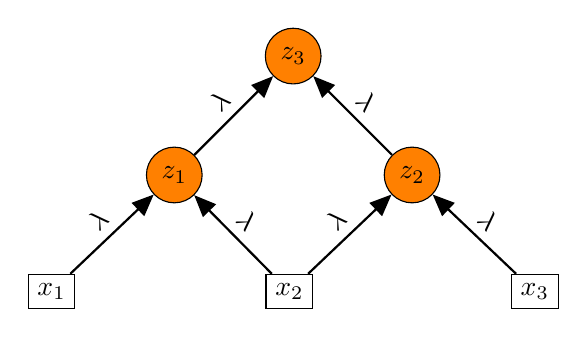
\begin{tikzpicture}
\node[draw, circle, fill=orange] (z3) {$ z_{3} $};

\node[draw, circle, fill=orange, below left =of z3] (z1) {$ z_{1} $};
\node[draw, circle, fill=orange, below right = of z3] (z2) {$ z_{2} $};

\node[draw, rectangle,  below left= of z1] (in1) {$ x_{1} $};
\node[draw, rectangle, below left=of z2] (in2) {$ x_{2} $}; 
\node[draw, rectangle, below right= of z2] (in3) {$ x_{3} $};

\pause
\draw[->, thick] (in1) -- (z1) node[midway, above, rotate=45] {$ \lambda $};
\draw[->, thick] (in2) -- (z1) node[midway, above, rotate=315] {$ \lambda $};
\draw[->, thick] (in2) -- (z2) node[midway, above, rotate=45] {$ \lambda $};
\draw[->, thick] (in3) -- (z2) node[midway, above, rotate=315] {$ \lambda $};
\pause
\draw[->, thick] (z1) -- (z3) node[midway, above, rotate=45] {$ \lambda $};
\draw[->, thick] (z2) -- (z3) node[midway, above, rotate=315] {$ \lambda $};
\end{tikzpicture}
\end{figure}
\end{frame}

\begin{frame}{Wake Phase Update}
\begin{figure}
\center
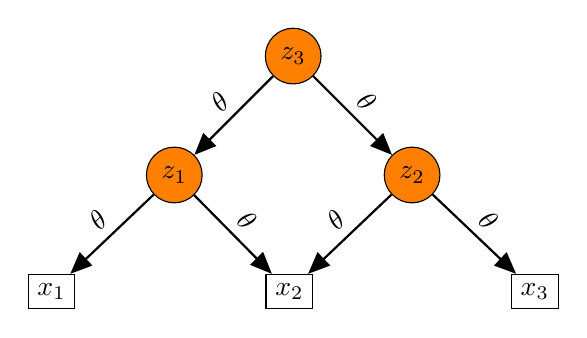
\begin{tikzpicture}
\node[draw, circle, fill=orange] (z3) {$ z_{3} $};

\node[draw, circle, fill=orange, below left =of z3] (z1) {$ z_{1} $};
\node[draw, circle, fill=orange, below right = of z3] (z2) {$ z_{2} $};

\node[draw, rectangle,  below left= of z1] (in1) {$ x_{1} $};
\node[draw, rectangle, below left=of z2] (in2) {$ x_{2} $}; 
\node[draw, rectangle, below right= of z2] (in3) {$ x_{3} $};

\draw[->, thick] (z1) -- (in1) node[midway, above, rotate=45] {$ \theta $};
\draw[->, thick] (z1) -- (in2) node[midway, above, rotate=315] {$ \theta $};
\draw[->, thick] (z2) -- (in2) node[midway, above, rotate=45] {$ \theta $};
\draw[->, thick] (z2) -- (in3) node[midway, above, rotate=315] {$ \theta $};
\draw[->, thick] (z3) -- (z1) node[midway, above, rotate=45] {$ \theta $};
\draw[->, thick] (z3) -- (z2) node[midway, above, rotate=315] {$ \theta $};
\end{tikzpicture}
\end{figure}
\end{frame}

\begin{frame}{Sleep Phase Objective}
Needed to find alternative objective because
$$ \pdv{\lambda} \E[q(z|x, \lambda)]{p(x,z|\theta)} = \sum_{z}\pdv{\lambda}q(z|x, \lambda)p(x,z|\theta) $$
is not an expectation!
\pause
\begin{block}{Idea}
Optimize $ q $ towards a sample from $ p $.
\end{block}

\end{frame}


\begin{frame}{Sleep Phase Objective}
Assumes fake data $ \tilde{x} $ and latent variables $ z $ to be fixed random draw from $ p(x,z|\theta) $.
\begin{equation*}
\begin{aligned}
&\max_{\lambda}~  \E[p(\tilde x, z|\theta)]{\log q(z|\tilde x, \lambda)} + \mathbb E_{p(\tilde x)}\left[\Ent{p(z|\tilde{x},\theta)}\right] \pause \\
&\overset{\text{MC}}{\approx} \max_{\lambda}~ \frac{1}{S}\sum_{s=1}^{S} \log q(z^{(s)}|\tilde{x}^{(s)}, \lambda),~~~ (\tilde{x},z)^{(s)} \sim p(x,z|\theta)
\end{aligned}
\end{equation*} 

\end{frame}

\begin{frame}{Sleep Phase Sampling}
\begin{figure}
\center
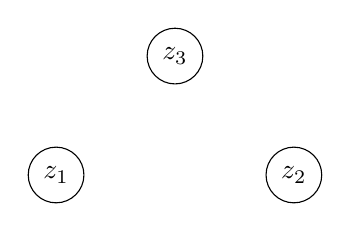
\begin{tikzpicture}
\node[draw, circle] (z3) {$ z_{3} $};

\node[draw, circle, below left =of z3] (z1) {$ z_{1} $};
\node[draw, circle, below right = of z3] (z2) {$ z_{2} $};
\end{tikzpicture}
\end{figure}
\end{frame}

\begin{frame}{Sleep Phase Sampling}
\begin{figure}
\center
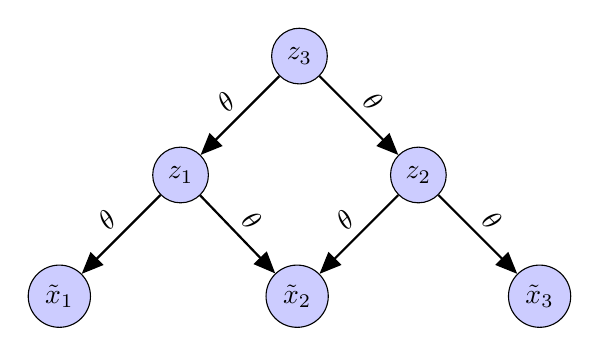
\begin{tikzpicture}
\node[draw, circle, fill=blue!20] (z3) {$ z_{3} $};

\node[draw, circle, fill=blue!20, below left =of z3] (z1) {$ z_{1} $};
\node[draw, circle, fill=blue!20, below right = of z3] (z2) {$ z_{2} $};

\node[draw, circle, fill=blue!20, below left= of z1] (in1) {$ \tilde{x}_{1} $};
\node[draw, circle, fill=blue!20, below left=of z2] (in2) {$ \tilde{x}_{2} $}; 
\node[draw, circle, fill=blue!20, below right= of z2] (in3) {$ \tilde{x}_{3} $};

\pause
\draw[->, thick] (z3) -- (z1) node[midway, above, rotate=45] {$ \theta $};
\draw[->, thick] (z3) -- (z2) node[midway, above, rotate=315] {$ \theta $};
\pause
\draw[->, thick] (z1) -- (in1) node[midway, above, rotate=45] {$ \theta $};
\draw[->, thick] (z1) -- (in2) node[midway, above, rotate=315] {$ \theta $};
\draw[->, thick] (z2) -- (in2) node[midway, above, rotate=45] {$ \theta $};
\draw[->, thick] (z2) -- (in3) node[midway, above, rotate=315] {$ \theta $};
\end{tikzpicture}
\end{figure}
\end{frame}

\begin{frame}{Sleep Phase Update}
\begin{figure}
\center
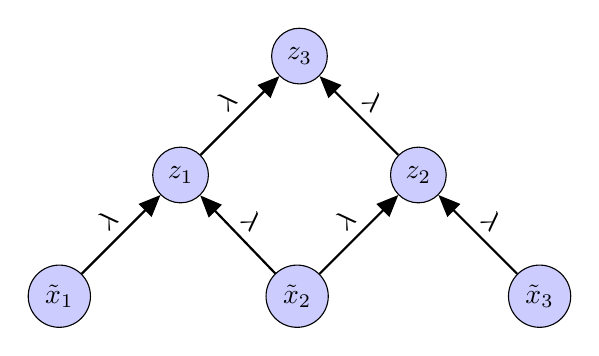
\begin{tikzpicture}
\node[draw, circle, fill=blue!20] (z3) {$ z_{3} $};

\node[draw, circle, fill=blue!20, below left =of z3] (z1) {$ z_{1} $};
\node[draw, circle, fill=blue!20, below right = of z3] (z2) {$ z_{2} $};

\node[draw, circle, fill=blue!20, below left= of z1] (in1) {$ \tilde{x}_{1} $};
\node[draw, circle, fill=blue!20, below left=of z2] (in2) {$ \tilde{x}_{2} $}; 
\node[draw, circle, fill=blue!20, below right= of z2] (in3) {$ \tilde{x}_{3} $};

\draw[->, thick] (in1) -- (z1) node[midway, above, rotate=45] {$ \lambda $};
\draw[->, thick] (in2) -- (z1) node[midway, above, rotate=315] {$ \lambda $};
\draw[->, thick] (in2) -- (z2) node[midway, above, rotate=45] {$ \lambda $};
\draw[->, thick] (in3) -- (z2) node[midway, above, rotate=315] {$ \lambda $};
\draw[->, thick] (z1) -- (z3) node[midway, above, rotate=45] {$ \lambda $};
\draw[->, thick] (z2) -- (z3) node[midway, above, rotate=315] {$ \lambda $};
\end{tikzpicture}
\end{figure}
\end{frame}

\begin{frame}{Wake-sleep Algorithm}
\textbf{Advantages}
\begin{itemize}
\item Simple layer-wise updates
\item Amortised inference: all latent variables are inferred from the same weights $ \lambda $
\end{itemize}
\pause
\textbf{Drawbacks}
\begin{itemize}
\item Inference and generative networks are trained on different objectives
\item Inference weights $ \lambda $ are updated on fake data $ \tilde{x} $
\item Generative weights are bad initially, giving wrong signal to the updates of $ \lambda $
\end{itemize}
\end{frame}

%\begin{frame}{What we know so far}
%\begin{itemize}
%\item Deep Generative Models are probabilistic models where the parameters of the conditional
%distributions are computed by neural networks
%\pause
%\item Because the $ \ELBO $ cannot be computed exactly, we need to sample latent values
%\pause
%\item Main problem: the MC estimator is not differentiable
%\pause
%\item Solution: reparametrisation gradient
%\end{itemize}
%\end{frame}
%
%\begin{frame}{Reparametrisation Gradient}
%\begin{block}{Model Gradient}
%\begin{equation*}
%\frac{\partial}{\partial \theta}\E[q(z|\lambda)]{\log p(x|z,\theta)} - \frac{\partial}{\partial \theta}\KL{q(z|\lambda)}{p(z|\theta)}
%\end{equation*}
%\end{block}
%\pause
%\begin{block}{Inference Network Gradient}
%\begin{equation*}
%\frac{\partial}{\partial \lambda}\E[q(z|\lambda)]{\log p(x|z,\theta)} - \frac{\partial}{\partial \lambda}\KL{q(z|\lambda)}{p(z|\theta)}
%\end{equation*}
%\end{block}
%\end{frame}
%
%\begin{frame}{Reparametrisation Gradient}
%\begin{equation*}
%\begin{aligned}
%&\frac{\partial}{\partial \lambda}\E[q(z|\lambda)]{\log p(x|z,\theta)} &= \\
%\pause
%&\frac{\partial}{\partial \lambda}\E[\phi(\epsilon)]{\log p(x|\overbrace{h^{-1}(\epsilon, \lambda)}^{z},\theta)} &= \\
%\pause
%&\E[\phi(\epsilon)]{\frac{\partial}{\partial z}\log p(x|\overbrace{h^{-1}(\epsilon, \lambda)}^{z},\theta) \times \frac{\partial}{\partial \lambda}
%\overbrace{h^{-1}(\epsilon, \lambda)}^{z}} &
%\end{aligned}
%\end{equation*}
%\end{frame}
%
%\begin{frame}
%\tableofcontents
%\end{frame}

%\section{Reparametrisation for Discrete Variables?}
%\begin{frame}
%\tableofcontents[currentsection]
%\end{frame}
%
%\begin{frame}{Reparametrisation}
%In order to tranform variables, we need to compute the Jacobian (matrix of partial derivatives).
%\begin{equation*}
%p(z) = p(\overbrace{h(z)}^{\epsilon})\left|\det J_{h(z)}\right|
%\end{equation*}
%The Jacobian 
%\begin{equation}
%	J_{ij} = \pdv{h_i(z)}{z_j}
%\end{equation}
%is generally not available for discrete variables. 
%\end{frame}
%
%%\begin{frame}{Cumulative Distribution Function}
%%Insert picture here
%%\end{frame}
%
%\begin{frame}{Continuity}
%The outcome space of discrete variables is non-continuous. Thus, we cannot take derivatives.
%\end{frame}

\section{Revisiting the Inference Gradient}
\begin{frame}
\tableofcontents[currentsection]
\end{frame}

\begin{frame}{Generative Model with NN Likelihood}
\begin{block}{Goal}
Define model $ p(x,z|\theta) = p(x|z,\theta)p(z) $ where the likelihood $ p(x|z,\theta) $ is given by a neural
network. (We fix $ p(z) $ for simplicity.)
\end{block}
\pause
\begin{block}{Problem}
$ p(x) = \intl{p(x|z,\theta) p(z)}{z} $ is hard to compute.
\end{block}
\end{frame}

\begin{frame}{Generative Model with NN Likelihood}
\begin{block}{Goal}
Define model $ p(x,z|\theta) = p(x|z,\theta)p(z) $ where the likelihood $ p(x|z,\theta) $ is given by a neural
network. (We fix $ p(z) $ for simplicity.)
\end{block}
\begin{block}{Problem}
$ p(x) = \intl{\alert{\underbrace{p(x|z,\theta)}_{\substack{\text{highly} \\  \text{non-linear!}}}} p(z)}{z} $ is hard to compute.
\end{block}
\end{frame}

\begin{frame}{Solution: Variational Inference}

\vspace{-10pt}
\begin{small}
\begin{equation*}
\begin{aligned}
\log p(x|\theta) &\geq \overbrace{\E[q(z|x, \lambda)]{\log p(x,Z|\theta)} + \Ent{q(z|x, \lambda)}}^{\ELBO} \\ 
\pause
&= \E[q(z|x, \lambda)]{\log p(x|Z, \theta) + \log p(Z)} + \Ent{q(z|x, \lambda)} \\ \pause
&= \E[q(z|x, \lambda)]{\log p(x|Z, \theta)} - \KL{q(z|x, \lambda)}{p(z)}
\end{aligned}
\end{equation*}
\end{small}

\pause

\vspace{-20pt}
\begin{equation*}
\argmax_{\theta,\lambda} ~ \E[q(z|x, \lambda)]{\log p(x|Z, \theta)} - \KL{q(z|x, \lambda)}{p(z)}
\end{equation*}


\pause

\begin{itemize}
	\item assume $\KL{q(z|x, \lambda)}{p(z)}$  analytical\\
	true for exponential families \pause
	\item approximate $\E[q(z|x, \lambda)]{\log p(x|z, \theta)}$ by sampling\\
	feasible because  $q(z|x, \lambda)$ is simple
\end{itemize}


\end{frame}

\begin{frame}{Generator Network Gradient}
\vspace{-10pt}
\begin{equation*}
\begin{aligned}
&\pdv{\theta}\E[q(z|x,\lambda)]{\log p(x|z,\theta)} - \overbrace{\KL{q(z|x,\lambda)}{p(z)}}^{constant} \\ \pause 
&=\E[q(z|x,\lambda)]{\pdv{\theta}\log p(x|z,\theta)} \\ \pause
&\overset{\text{MC}}{\approx} \frac{1}{S}\sum_{i=1}^{S}
\pdv{\theta} \log p(x|z_{i},\theta) \\
&\textcolor{gray}{\text{where }z_i \sim q(z|x, \lambda)}
\end{aligned}
\end{equation*}
\pause
\center{Note: $ q(z|x,\lambda) $ does not depend on $ \theta $.}
\end{frame}

\begin{frame}{Inference Network Gradient}
\begin{equation*}
\begin{aligned}
&\pdv{\lambda}\left[\E[q(z|x,\lambda)]{\log p(x|z,\theta)} - \KL{q(z|x,\lambda)}{p(z)} \right] \\ \pause
=&\pdv{\lambda}\E[q(z|x,\lambda)]{\log p(x|z,\theta)} - \underbrace{\pdv{\lambda}\KL{q(z|x,\lambda)}{p(z)}}_{\text{analytical computation}} \\
\end{aligned}
\end{equation*}
\pause
\center{The first term again requires approximation by sampling}
\end{frame}

\begin{frame}{Inference Network Gradient}

\begin{equation*}
\begin{aligned}
&\pdv{\lambda}\E[q(z|x,\lambda)]{\log p(x|z,\theta)} \\ \pause
&= \pdv{\lambda} \sum_{z}q(z|x,\lambda)\log p(x|z,\theta) \\ \pause
&= \sum_{z}\alert{\pdv{\lambda} q(z|x,\lambda)}\log p(x|z,\theta)
\end{aligned}
\end{equation*}
\pause
Not an expectation!
\end{frame}

\begin{frame}{Back to Basic Calculus}
\begin{equation*}
\dv{\lambda}\log f(\lambda) \pause = \frac{\dv{\lambda}f(\lambda)}{f(\lambda)}
\end{equation*}
\pause
\begin{block}{Consequence}
\begin{equation*}
\dv{\lambda}f(\lambda) = \textcolor{blue}{\dv{\lambda}\log f(\lambda) \times f(\lambda)}
\end{equation*}
\end{block}
\end{frame}

\begin{frame}{Score Function Estimator}
\begin{equation*}
\dv{\lambda}f(\lambda) = \textcolor{blue}{\dv{\lambda}\log f(\lambda) \times f(\lambda)}
\end{equation*}
\pause
Apply this to the ELBO derivative.
\begin{equation*}
\begin{aligned}
&\sum_{z}\textcolor{blue}{\frac{\partial}{\partial \lambda}q(z|\lambda)}\times\log p(x|z,\theta) = \\
\pause
&\sum_{z}\textcolor{blue}{q(z|\lambda)\frac{\partial}{\partial \lambda}\log q(z|\lambda)} \times \log p(x|z,\theta) = \\
\pause
&\E[q(z|\lambda)]{\frac{\partial}{\partial \lambda}\log q(z|\lambda) \times \log p(x|z,\theta)}
\end{aligned}
\end{equation*}
\end{frame}

%\begin{frame}{Comparison Between Estimators}
%\begin{itemize}
%\item Score function gradient
%\begin{equation*}
%\E[q(z|\lambda)]{\frac{\partial}{\partial \lambda}\log q(z|\lambda) \times \log p(x|z,\theta)}
%\end{equation*}
%\item Reparametrisation gradient
%\begin{equation*}
%\E[\phi(\epsilon)]{\frac{\partial}{\partial \lambda} \log p(x|h^{-1}(\epsilon, \lambda),\theta)}
%\end{equation*}
%\end{itemize}
%\end{frame}

\begin{frame}{Example Model}
Let us consider a latent factor model for topic modelling. Each document $ x $ consists of $ n $ i.i.d.
categorical draws from that model. The categorical distribution in turn depends on the binary latent 
factors $ z = (z_{1},\ldots,z_{k}) $ which are also i.i.d.
\begin{equation*}
\begin{aligned}
Z_{j} &\sim \BerDist{\phi} && (1 \leq j \leq k) \\ 
X_{i}|z &\sim \CatDist{g(z)} && (1 \leq i \leq n)
\end{aligned}
\end{equation*} 
Here $ g(\cdot) $ is a function computed by neural network with softmax output.
\end{frame}

\begin{frame}{Example Model}
\begin{figure}
\center
\begin{tikzpicture}
\foreach \x in {1,...,4} {
  \pgfmathtruncatemacro{\y}{\x-1}
  \ifthenelse{\x=1}{\node[obs] (x\x) {$ x_{\x} $}}{\node[obs, right= of x\y] (x\x) {$ x_{\x} $}};
}
\foreach \z in {1,2,3} {
  \node[latent, above right = of x\z] (z\z) {$ z_{\z} $};
  \edge{z\z}{x1,x2,x3,x4};
}
\end{tikzpicture}
\end{figure}
At inference time the latent variables are marginally dependent. For our variational distribution
we are going to assume that they are not (recall: mean field assumption).
\end{frame}

\begin{frame}{Inference Network}
\begin{figure}
\center
\begin{tikzpicture}
\foreach \x in {1,...,4} {
\pgfmathtruncatemacro{\y}{\x-1}
\ifthenelse{\x=1}{\node[obs] (x\x) {$ x_{\x} $}}{\node[obs, right= of x\y] (x\x) {$ x_{\x} $}};
}
\foreach \z in {1,2,3} {
  \node[latent, above right = of x\z] (z\z) {$ z_{\z} $};
  \edge[color=red]{x1,x2,x3,x4}{z\z};
}
\end{tikzpicture}
\end{figure}
The inference network needs to predict $ k $ Bernoulli parameters $ \psi $. Any neural network with
sigmoid output will do that job.
\end{frame}

\begin{frame}{Computation Graph}
\begin{figure}
\center
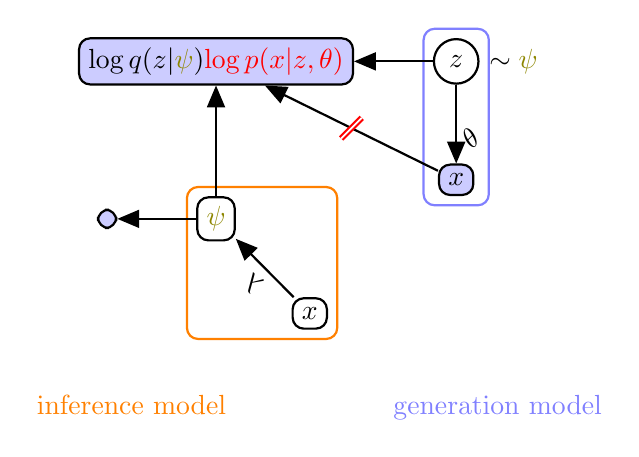
\begin{tikzpicture}[node distance=1cm]
\node[rectangle, draw, rounded corners, thick] (input) {$x$};
\node[rectangle, draw, rounded corners, thick, above left=of input] (psi) {$ \textcolor{olive}{\psi} $};
\draw[->, thick] (input) -- (psi) node[midway, above, rotate=145] {$ \lambda $};
\node[draw=orange, thick, rectangle, fit= (input) (psi), rounded corners] {};
\node[below left= of input] (inference) {\textcolor{orange}{inference model}};

\pause
\node[rectangle, draw, fill=blue!20, thick, rounded corners, thick, left=of psi] (kl) {$ \KullbackLeibler $};
\draw[->, thick] (psi) edge (kl);

\pause
\node[rectangle, fill=blue!20, thick, above of= psi, rounded corners, draw, node distance=2cm] (scorefunction) {$ \log q(z|\textcolor{olive}{\psi}) \textcolor{red}{\log p(x|z,\theta)} $};
\draw[->, thick] (psi) edge (scorefunction);

\pause
\node[circle, draw, thick, right= of scorefunction] (z) {$ z $};
\node[rectangle, fill=blue!20, thick, below = of z, rounded corners, draw] (loss) {$ x $};
\node[draw=blue!50, thick, rectangle, fit= (z) (loss), rounded corners] {};
\node[below right= of input] (generation) {\textcolor{blue!50}{generation model}};
\node[right = of z, xshift=-1cm] (random) {$ \sim \BerDist{\textcolor{olive}{\psi}} $};
\draw[->, thick] (z) -- (loss) node[midway, above, rotate=225] {$ \theta $};
\draw[->, thick] (z) edge (scorefunction);
\draw[->, thick] (loss) edge node[strike out,draw,-,red,double]{} (scorefunction);
\end{tikzpicture}
\end{figure}
\end{frame}

%\begin{frame}{Reparametrisation Gradient}
%\begin{figure}
%\center
%\begin{tikzpicture}[node distance=1cm]
%\node[rectangle, draw, rounded corners, thick] (input) {$x$};
%\node[rectangle, draw, rounded corners, thick, above left=of input] (mu) {$ \mu $};
%\node[rectangle, draw, rounded corners, thick, above right=of input] (var) {$ \sigma $};
%\node[rectangle, draw, rounded corners, thick, above right= of mu] (z) {$ z $};
%\node[rectangle, fill=blue!20, thick, above of= z, rounded corners, draw, node distance=1.5cm] (output) {$ x $};
%
%\draw[->, thick] (input) -- (mu) node[midway, above, rotate=315] {$ \lambda $};
%\draw[->, thick] (input) -- (var) node[midway, above, rotate=45] {$ \lambda $};
%\draw[->, thick] (mu) edge (z);
%\draw[->, thick] (var) edge (z);
%\draw[->, thick] (z) -- (output) node[midway, right] {$ \theta $};
%
%\node[draw=orange, thick, rectangle, fit= (input) (mu) (var), rounded corners] {};
%\node[left= of mu] (inference) {\textcolor{orange}{inference model}};
%
%\node[draw=blue!50, thick, rectangle, fit= (z) (output), rounded corners] {};
%\node[above= of inference] (generation) {\textcolor{blue!50}{generation model}};
%
%\node[circle, draw, thick ,right =of var, xshift=-.5cm] (epsilon) {$ \epsilon $};
%\node[right = of epsilon, xshift=-1cm] (stdNormal) {$ \sim \NDist{0}{1} $};
%\draw[->, thick] (epsilon) edge (var);
%
%\node[above= of mu, rectangle, draw, fill=blue!20, thick, rounded corners, thick] (KLmu) {$ \KullbackLeibler $};
%\draw[->, thick] (mu) edge (KLmu);
%\node[above= of var, rectangle, draw, fill=blue!20, thick, rounded corners, thick] (KLvar) {$ \KullbackLeibler $};
%\draw[->, thick] (var) edge (KLvar);
%\end{tikzpicture}
%\end{figure}
%\end{frame}

\begin{frame}{Pros and Cons}
\begin{itemize}
\item Pros
\begin{itemize}
\item Applicable to all distributions
\item Many libraries come with samplers for common distributions
\end{itemize}
\pause
\item Cons
\begin{itemize}
\item High Variance!
\end{itemize}
\end{itemize}
\end{frame}

\section{Control Variates and Baselines}

\begin{frame}
\tableofcontents[currentsection]
\end{frame}

\begin{frame}{Baselines}
\begin{block}{Fact}
The Expectation of the score function is 0. 
\pause
\begin{equation*}
\E[q(z|x,\lambda)]{\pdv{\lambda} \log q(z|x,\lambda)} = 0
\end{equation*}
\end{block}
\end{frame}

\begin{frame}{Baselines}
We attempt to centre the gradient estimate. To do this we learn a quantity $ C $ that we subtract
from the reconstruction loss.
\begin{equation*}
\E[q(z|\lambda) ]{\log q(z|\lambda) \left( \log p(x|z,\theta) - C \right)}
\end{equation*}
We call $ C $ a baseline. It does not change the expected gradient \citep{Williams:1992}.
\end{frame}

\begin{frame}{Baselines}
 \begin{equation*}
\begin{aligned}
&\E[q(z|\lambda)]{\pdv{\lambda}\log q(z|\lambda) \left( \log p(x|z,\theta) - C \right)} = \pause \\
&\underbrace{\E[q(z|\lambda)]{\pdv{\lambda}\log q(z|\lambda)  \log p(x|z,\theta)}}_{\text{score function gradient}}  -
\pause \\
&\underbrace{\E[q(z|\lambda)]{\pdv{\lambda}\log q(z|\lambda)}}_{0}C
\end{aligned}
\end{equation*}
\end{frame}

\begin{frame}{Baselines}
We can make baselines input-dependent to make them more flexible.
\begin{equation*}
\log q(z|\lambda) \left( \log p(x|z,\theta) - C(x; \omega) \right)
\end{equation*}

\pause

However, baselines may not depend on the random value $ z $! Quantities that may depend on the
random value ($ C(z) $) are called \textbf{control variates}. \\

~

See \cite{PaisleyEtAl:2012, RanganathEtAl:2014,GregorEtAl:2014}.
\end{frame}

\begin{frame}{Baselines}
Baselines are predicted by a regression model (e.g. a neural net). \\

~

The model is trained using 
an $ L_{2} $-loss.
\begin{equation*}
\min_\omega \left(C(x; \omega) - \log p(x|z,\theta)\right)^{2}
\end{equation*}
\end{frame}

\begin{frame}{Summary}
\begin{itemize}
\pause
\item Differentiating ELBO wrt $ \lambda $ does not yield an expectation.
\pause
\item Use score function estimator.
\pause
\item High variance.
\pause
\item Always use baselines for variance reduction!
\end{itemize}
\end{frame}

%\section{Semisupervised Learning}
%
%\begin{frame}{Putting it all together}
%We now know how to handle continuous and discrete latent variables. Let us combine these two treat partially observed data.
%\pause
%\begin{block}{Morphological Reinflection}
%Transform an inflected form of a verb into another.
%\begin{itemize}
%\pause
%\item plays $ \rightarrow $ played
%\pause
%\item walking $ \rightarrow $ walks
%\end{itemize}
%\end{block}
%\end{frame}
%
%\begin{frame}{A Simple Model \citep{ZhouNeubig:2017}}
%What do we need to correctly inflect a word?
%\pause
%\begin{itemize}
%\item lemma \pause (real vector)
%\pause
%\item morphological information \pause (discrete vector)
%\end{itemize}
%\end{frame}
%
%\begin{frame}{A Simple Model \citep{ZhouNeubig:2017}}
%\begin{figure}
%\center
%\begin{tikzpicture}
%\node[obs] (input) {$t$};
%\node[latent, above left = of input] (lemma) {$ z $};
%\node[circle, above right = of input, pattern=stripes, draw=black, pattern color=gray!25, radius=1cm] (morph)  {$ y $};
%\node[obs, left = of lemma] (base) {$ s $};
%\edge{lemma, morph}{input};
%\end{tikzpicture}
%\end{figure}
%\begin{itemize}
%\item $ z $ = lemma (continuous)
%\item $ y $ = morphological features (discrete)
%\item $ s $ = source form (inflected)
%\item $ t $ = target form (inflected)
%\end{itemize}
%\end{frame}
%
%\begin{frame}{A Simple Model \citep{ZhouNeubig:2017}}
%\begin{figure}
%\center
%\begin{tikzpicture}
%\node[obs] (input) {$t$};
%\node[latent, above left = of input] (lemma) {$ z $};
%\node[circle, above right = of input, pattern=stripes, draw=black, pattern color=gray!25, radius=1cm] (morph)  {$ y $};
%\node[obs, left = of lemma] (base) {$ s $};
%\edge{lemma, morph}{input};
%\path (input) edge[bend right=45, color=red, ->, thick] (morph);
%\path (base) edge[color=red, ->, thick] (lemma);
%\end{tikzpicture}
%\end{figure}
%\begin{itemize}
%\item $ z $ = lemma (continuous)
%\item $ y $ = morphological features (discrete)
%\item $ s $ = source form (inflected)
%\item $ t $ = target form (inflected)
%\end{itemize}
%\end{frame}
%
%\begin{frame}{A Simple Model \citep{ZhouNeubig:2017}}
%\begin{figure}
%\center
%\begin{tikzpicture}
%\node[obs] (input) {$t$};
%\node[latent, above left = of input] (lemma) {$ z $};
%\node[circle, above right = of input, pattern=stripes, draw=black, pattern color=gray!25, radius=1cm] (morph)  {$ y $};
%\node[obs, left = of lemma] (base) {$ s $};
%\edge{lemma, morph}{input};
%\path (input) edge[bend right=45, color=red, ->, thick] (morph);
%\path (base) edge[color=red, ->, thick] (lemma);
%\path (lemma) edge[color=green, ->, thick] (morph);
%\end{tikzpicture}
%\end{figure}
%\begin{itemize}
%\item $ z $ = lemma (continuous)
%\item $ y $ = morphological features (discrete)
%\item $ s $ = source form (inflected)
%\item $ t $ = target form (inflected)
%\end{itemize}
%\end{frame}

\begin{frame}[allowframebreaks]
\bibliographystyle{plainnat}
\bibliography{../../VI}
\end{frame}

\end{document}